% \textbf{\underline{OZ 6 - Magnetische inductie en de wet van Faraday - Oefening 5:}}
% \vspace{0.5cm}

% Een kort stuk van een draad, van lengte $ a $, beweegt met snelheid $ \vec{v} $, parallel langs een zeer lange draad waardoor een stroom $ I $ loopt (Figuur 6.5). Het dichtste uiteinde van de korte draad is een afstand $ b $ van de lange draad verwijderd. Neem aan dat de verticale draad lang is vergeleken met $ a + b $. Bepaal de emf tussen de uiteinde van de korte draad wanneer $ \vec{v} $

% \begin{enumerate}[(a)]
%     \item in de zelfde zin is als $ I $.
%     \item in de tegengestelde zin is als $ I $.
% \end{enumerate}

% \begin{figure}[H]
%     \centering
%     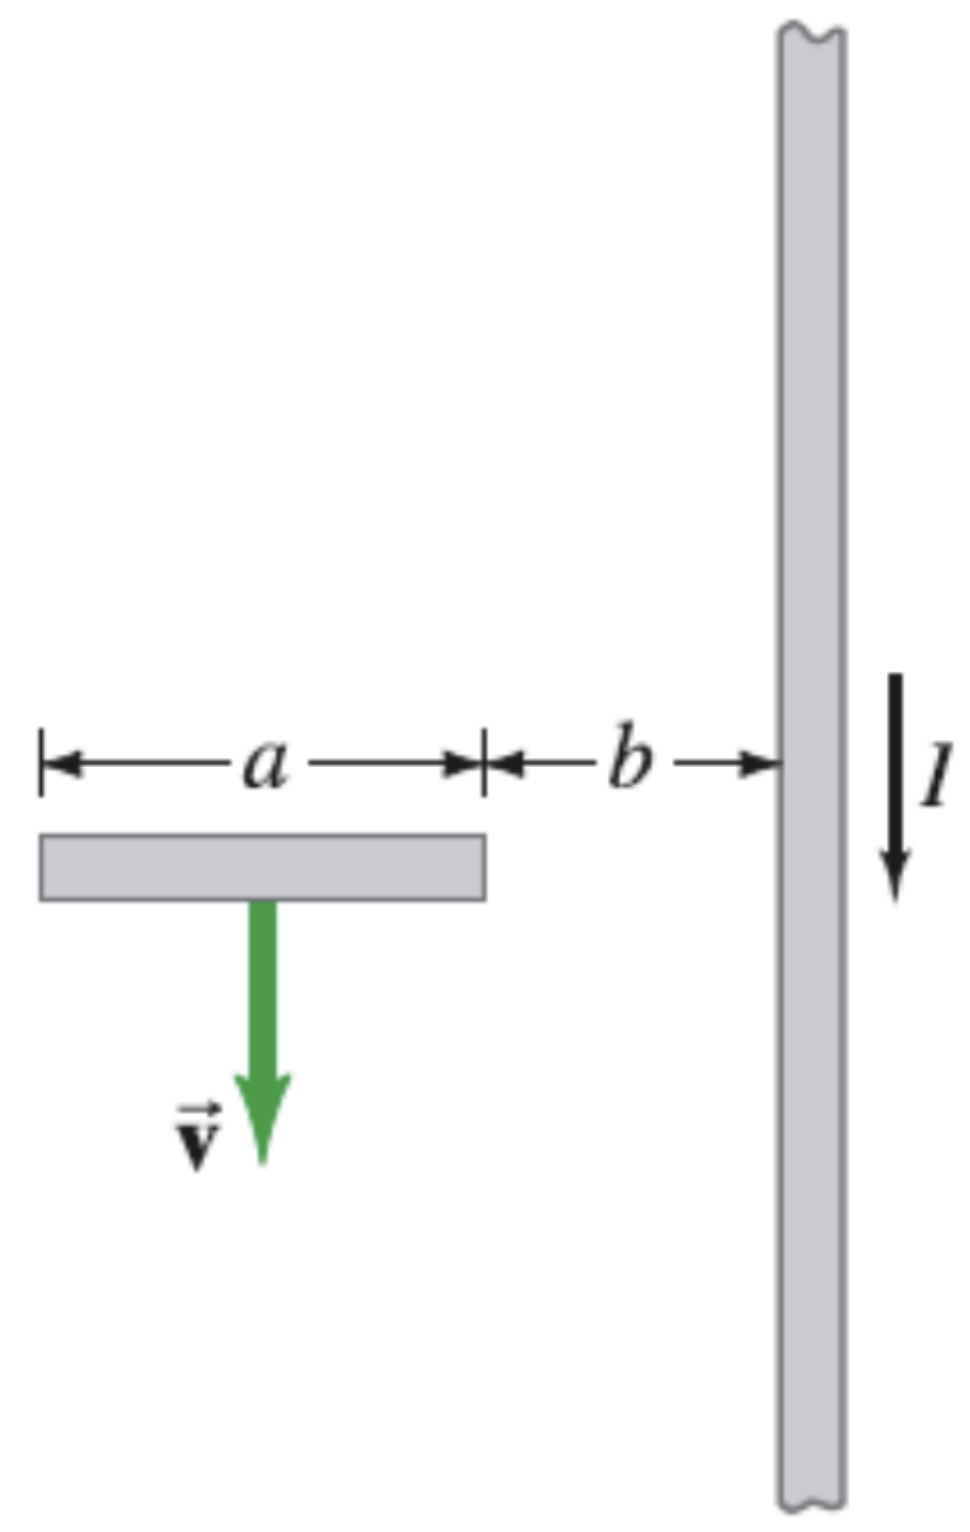
\includegraphics[width=4cm]{oz06/resources/oef-5-opgave.png}
    
%     \textbf{Figuur 6.5}
% \end{figure}


% \begin{description}[labelwidth=1.5cm, leftmargin=!]
%     \item[Geg. :]  
%     \item[Gevr. :]  
%     \item[Opl. :] (Oplossing van Serway 6E Chapter 31 Problem 63, niet 100\% hetzelfde want enkel in zelfde richting wordt berekend)

%     Find an expression for the flux through a rectangular area "swept out" by the bar in time $t$. The magnetic field at a distance $x$ from wire is
%     \\\\
% $B=\frac{\mu_0 I}{2 \pi x}$ and $\Phi_B=\int B d A$. Therefore,
% \\\\
% $\Phi_B=\frac{\mu_0 I v t}{2 \pi} \int_r^{r+\ell} \frac{d x}{x}$ where $v t$ is the distance the bar has moved in time $t$.
% \\\\
% Then, $|\varepsilon|=\frac{d \Phi_B}{d t}=\frac{\mu_0 I v}{2 \pi} \ln \left(1+\frac{\ell}{r}\right)$.
    
% \end{description}


